\documentclass[crop=false, class=book]{standalone}

%impostazioni lingua
\usepackage[T1]{fontenc}
\usepackage[utf8]{inputenc}
\usepackage[english,italian]{babel}

\usepackage[dvipsnames]{xcolor}
\usepackage{listings}

\lstdefinelanguage{Kotlin}{
	comment=[l]{//},
	commentstyle={\color{gray}\ttfamily},
	emph={[1]first, firstOrNull, forEach, lazy, map, mapNotNull, println},
	emphstyle={[1]\color{OrangeRed}},
	identifierstyle=\color{black},
	keywords={!in, !is, abstract, actual, annotation, as, as?, break, by, catch, class, companion, const, constructor, continue, crossinline, data, delegate, do, dynamic, else, enum, expect, external, false, field, file, final, finally, for, fun, get, if, import, in, infix, init, inline, inner, interface, internal, is, lateinit, noinline, null, object, open, operator, out, override, package, param, private, property, protected, public, receiveris, reified, return, return@, sealed, set, setparam, super, suspend, tailrec, this, throw, true, try, typealias, typeof, val, var, vararg, when, where, while, it},
	keywordstyle={\color{NavyBlue}\bfseries},
	morecomment=[s]{/*}{*/},
	morestring=[b]",
	morestring=[s]{"""*}{*"""},
	ndkeywords={@Deprecated, @JvmField, @JvmName, @JvmOverloads, @JvmStatic, @JvmSynthetic, Array, Byte, Double, Float, Int, Integer, Iterable, Long, Runnable, Short, String, Any, Unit, Nothing, Config, LightEstimationMode, CameraConfigFilter, CameraConfig, FacingDirection, AugmentedFaceMode, AugmentedFace, TrackingState, RegionType, CloudAnchorMode,AugmentedImageDatabase, BitmapFactory, Session, InstantPlacementMode, File, Uri, RecordingConfig },
	ndkeywordstyle={\color{BurntOrange}\bfseries},
	sensitive=true,
	stringstyle={\color{ForestGreen}\ttfamily},
	emph={[2]FRONT,MESH3D,ENVIRONMENTAL\_HDR,AMBIENT\_INTENSITY, DISABLED,FOREHEAD\_LEFT,FOREHEAD\_RIGHT,NOSE\_TIP, TRACKING, ENABLED, LOCAL\_Y\_UP},
	emphstyle={[2]\color{Purple}\ttfamily},
}

\definecolor{lightgrey}{RGB}{230,237,244}

\lstset{
	basicstyle=\scriptsize\sffamily\color{black},
	backgroundcolor=\color{lightgrey},
	frame=single,
	numbers=left,
	numbersep=5pt,
	numberstyle=\tiny\color{gray},
	showspaces=false,
	showstringspaces=false,
	tabsize=1,
	texcl=true,
	captionpos=b,
	breaklines=true
}




%sistema i margini
\usepackage{geometry}
\geometry{a4paper,top=2.2cm,bottom=2.2cm,left=3cm,right=3cm, heightrounded}

%interlinea 1.5
\usepackage{setspace}
\onehalfspacing

%gestione delle testatine
\usepackage{fancyhdr}
\pagestyle{fancy}
\lhead{}
\chead{}
\rhead{Titolo}
\lfoot{}
\cfoot{\thepage}
\rfoot{}
\renewcommand{\headrulewidth}{0.4pt}

%formattazione titoli paragrafo
\usepackage{titlesec}
\titleformat{\chapter}[block]{\normalfont\huge\bfseries}{\thechapter.}{0.7em}{\huge}

%pacchetti per i riferimenti in bibliografia
\usepackage[autostyle,italian=guillemets]{csquotes}
\usepackage[style=numeric,citestyle=numeric-comp,backend=biber]{biblatex}

%risorsa che contiene la bibliografia
\addbibresource{./../bibliografia.bib}

\usepackage{lipsum}
\usepackage{graphicx}
\usepackage[italian]{varioref}
\usepackage{copyrightbox}

\begin{document}
		
	\chapter{Anchor Trackable}
	
		ARCore definisce gli Anchor per assicurare che gli oggetti virtuali rimangano nella stessa posizione e vengano 					tracciati nel tempo. L'ambiente circostante può cambiare ed è necessario che la posizione dell'oggetto virtuale 				relativa alla mappa rimanga stabile. Gli Anchor sono disposti in insieme di punti o piani rappresentati da oggetti di 			tipo Trackable. \\
		Su questi oggetti possono essere invocati 3 metodi:
		\begin{itemize}
			\item[•] \textbf{createAnchor(Pose pose)} crea un anchor in una posa che è definita nel Trackable corrente. Il tipo di oggetto Trackable definirà il modo con cui l'anchor verrà disposto e la modalità di aggiornamento della sua posa mentre ARCore cambia il suo modello del mondo.
			\item[•] \textbf{ getAnchors()} restituisce tutti gli anchor presenti nel dato Trackable.
			\item[•] \textbf{getTrackingState()} restituisce un oggetto TrackingState che rappresenta lo stato del Trackable. Questo stato può essere: PAUSED quando il rilevamento viene perso ma potrebbe riprendere in futuro; STOPPED quando viene fermato e non verrà più ripreso; TRACKING se viene tracciato il determinato Trackable.
		\end{itemize}

	\begin{flushleft}
		Un esempio di tracciamento si può trovare nella sezione \emph{AugmentedImages} della nostra applicazione in cui è stato 		usato il metodo TrackingState per controllare se l'immagine di un pianeta veniva tracciata. 		 			(Esempio\vref{lst:Definizione Anchor in Augmented Images})\\
		Nella modalità \emph{Plane Detection} gli anchor vengono disposti in Trackable che rappresentano i piani. Quando un animale viene posizionato in punto mantiene invariata la sua posa (posizione e orientamento) anche se l'ambiente circostante cambia. Ad esempio, se posizioniamo un animale nel nostro salotto, andiamo in cucina e ritorniamo in salotto, dobbiamo trovare l'animale nello stesso punto di prima.\\
		
		Di seguito sono riportati degli esempi in cui si può notare che la posizione del pinguino resta invariata da qualsiasi 			prospettiva (frontale,posteriore,laterale) e distanza.
	\end{flushleft}
	
	
	\clearpage
	\begin{figure}
			\centering
			\copyrightbox[0.5]{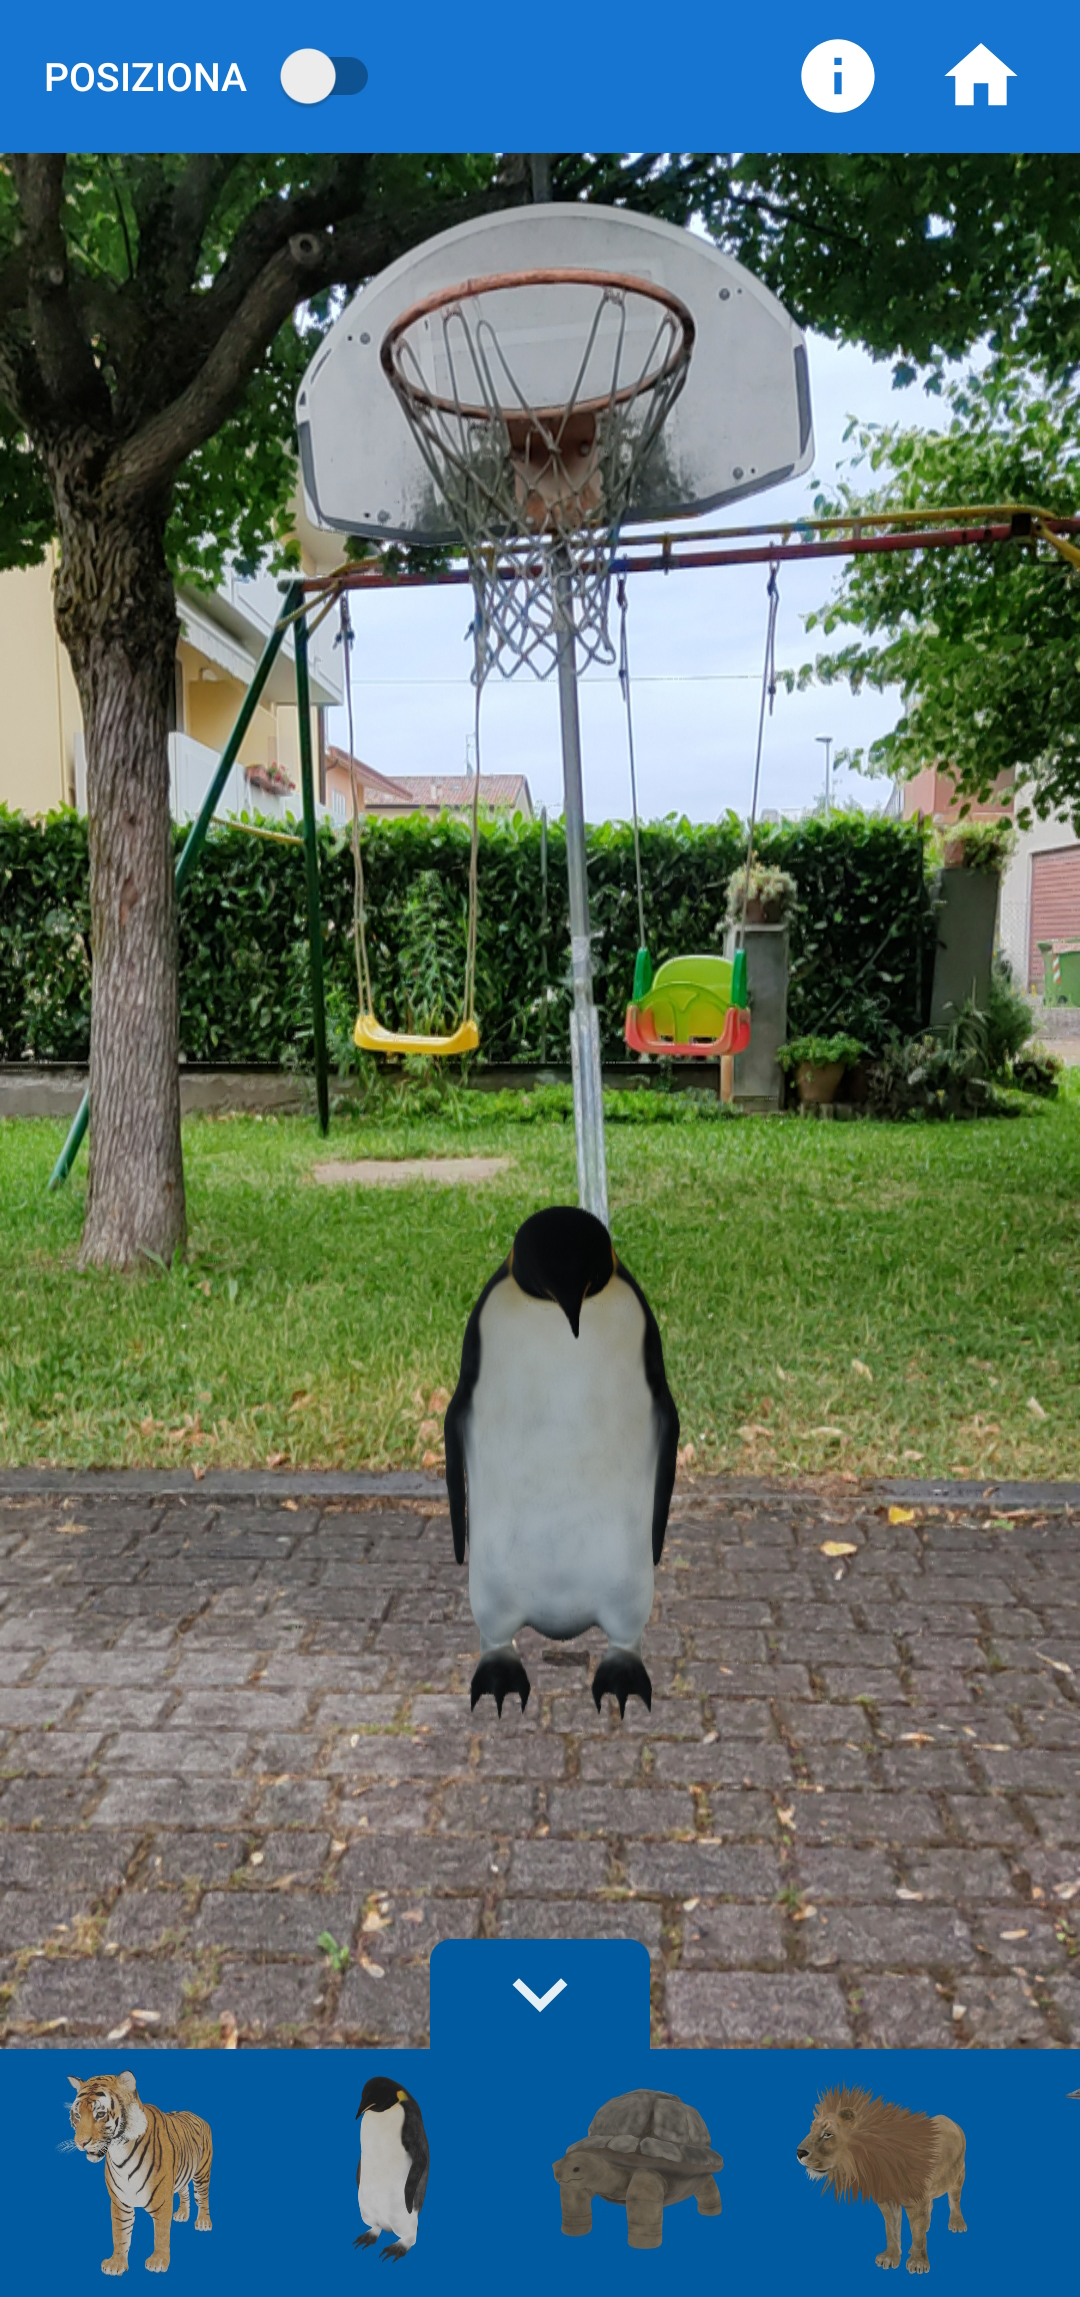
\includegraphics[width=0.3\textwidth]{../../resources/images/AnchorTrackable/pingvicino.jpg}}%
			{Fonte: \url{nostra applicazione}}
			\caption{Pinguino da un'inquadratura vicina}
			\label{fig: pinguino vicino}
	\end{figure}
	
	\begin{figure}
			\centering
			\copyrightbox[0.5]{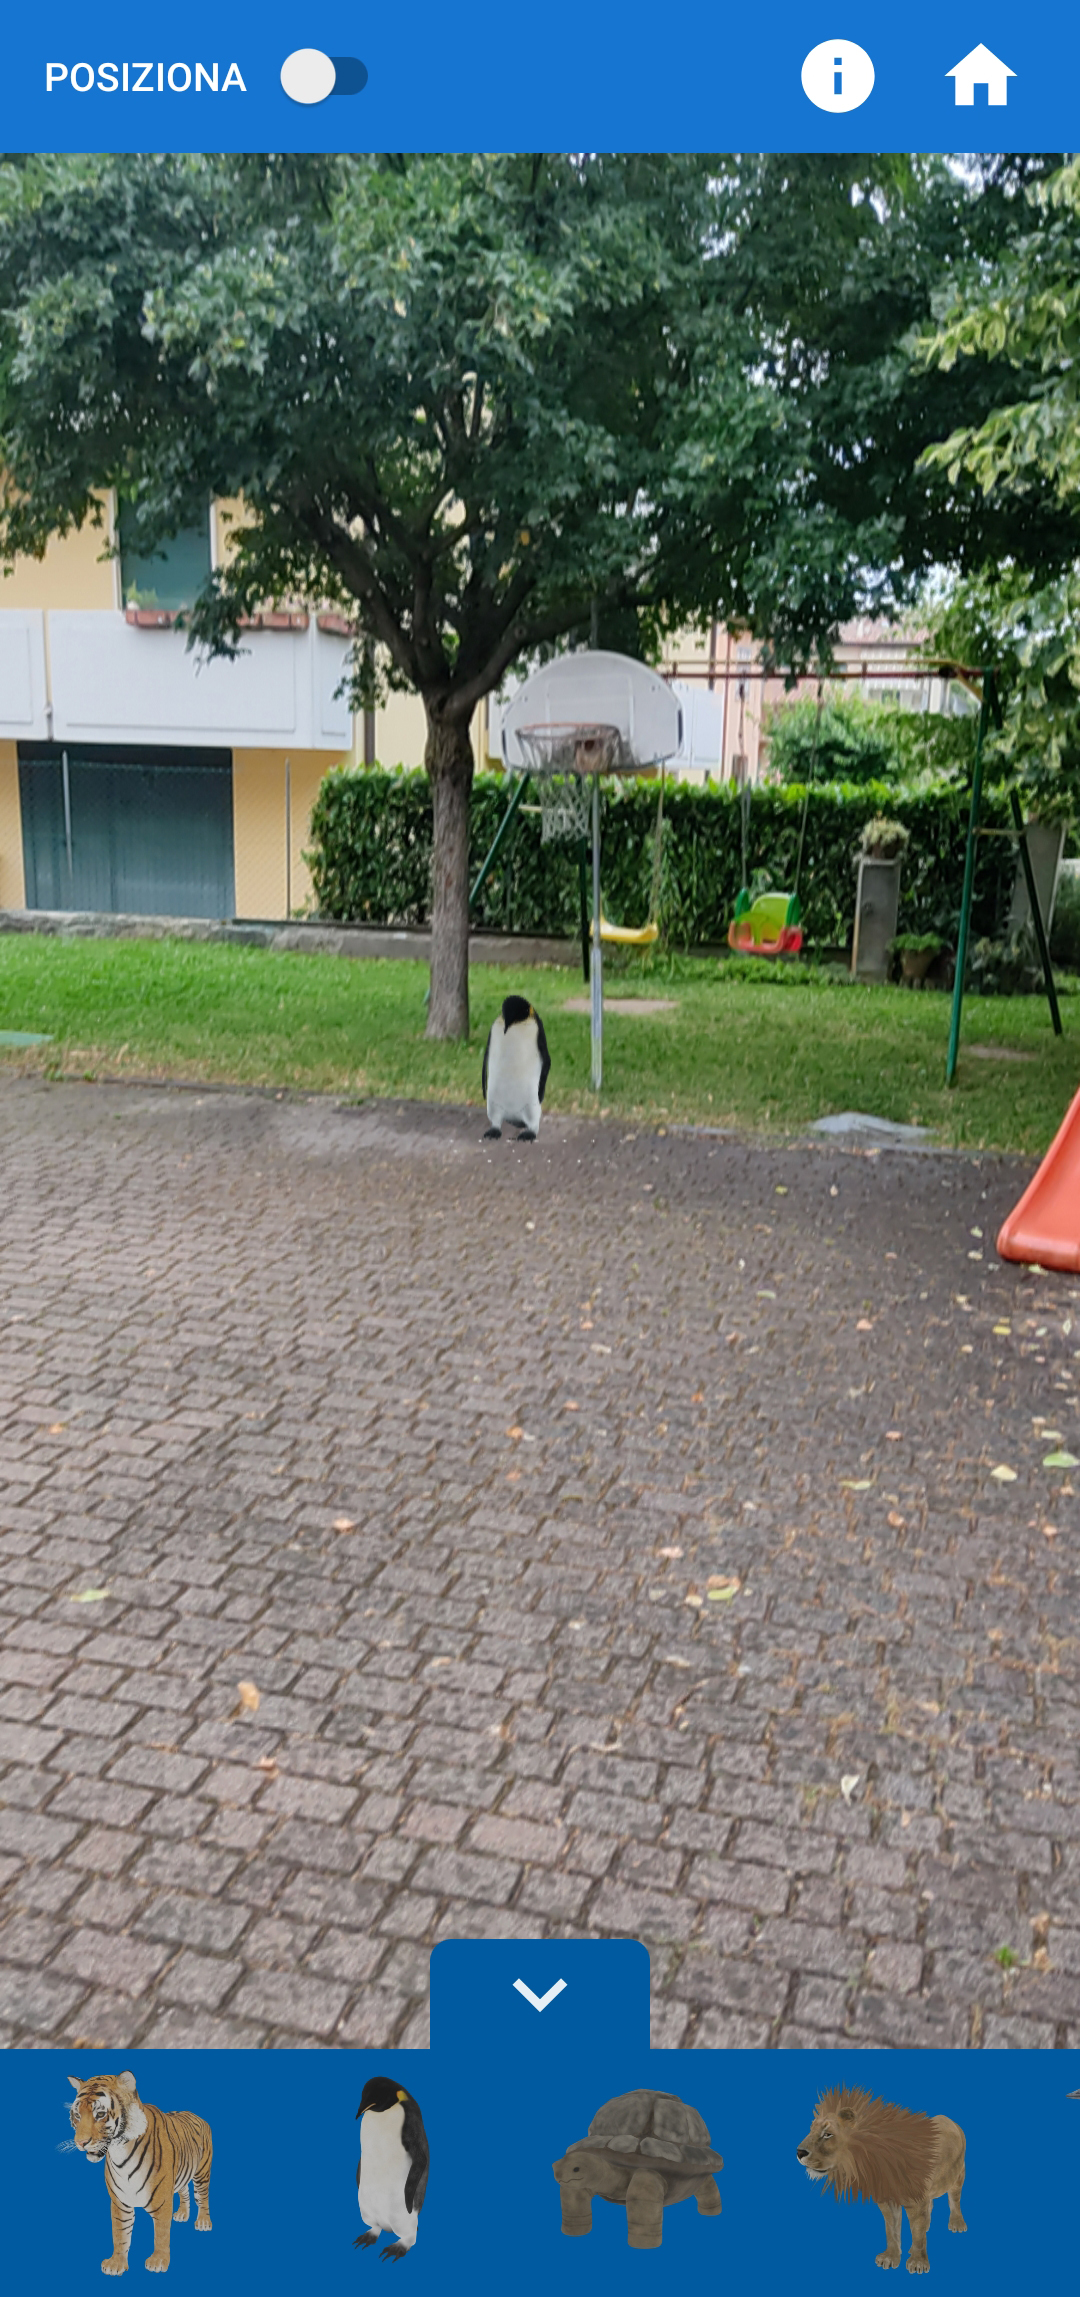
\includegraphics[width=0.3\textwidth]{../../resources/images/AnchorTrackable/pinglontano1.jpg}}%
			{Fonte: \url{nostra applicazione}}
			\caption{Pinguino da un'inquadratura lontana frontale}
			\label{fig: pinguino lontano1}
	\end{figure}
	
	\begin{figure}
			\centering
			\copyrightbox[0.5]{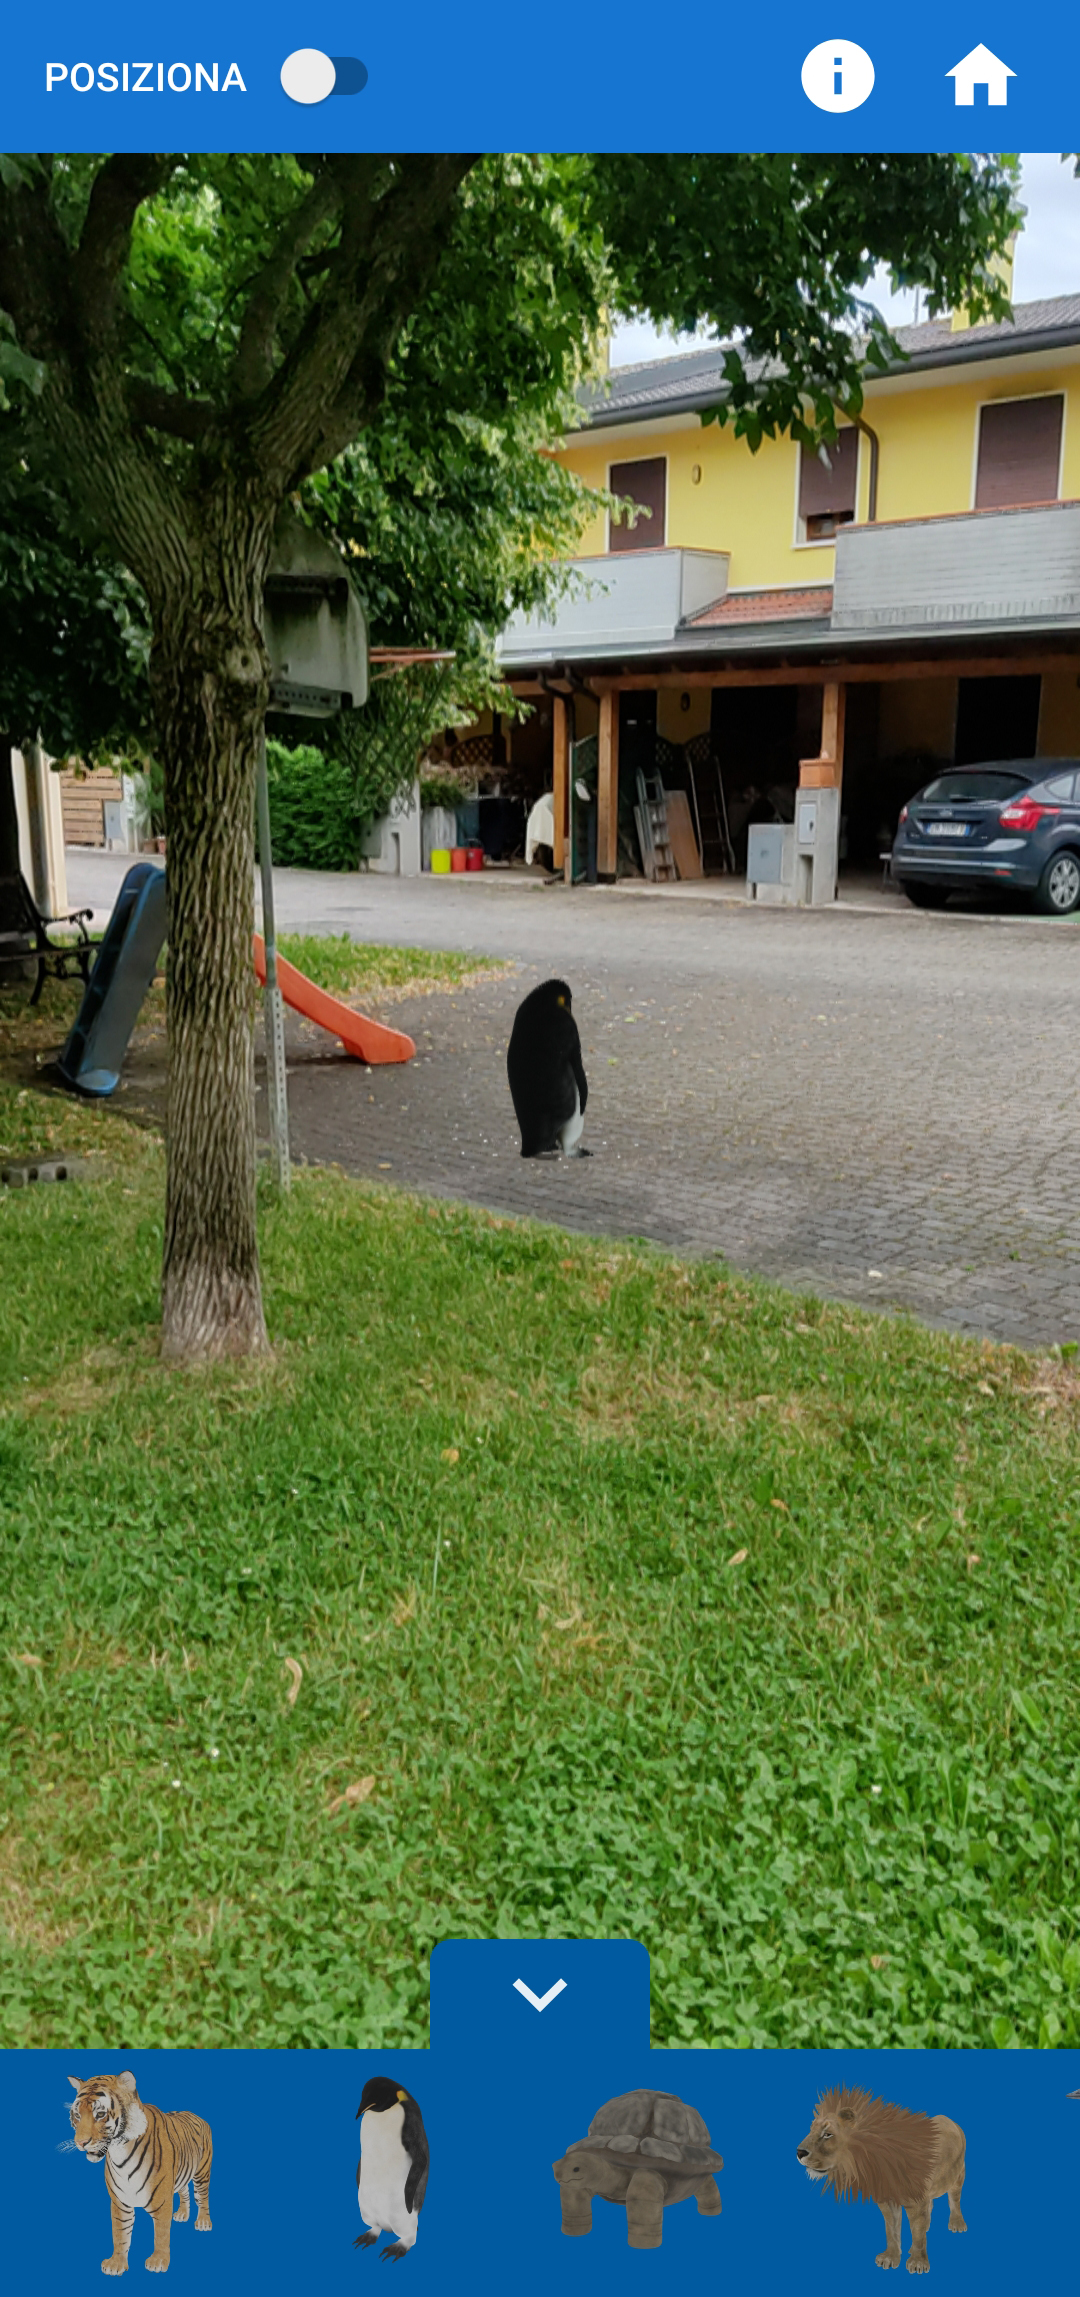
\includegraphics[width=0.3\textwidth]{../../resources/images/AnchorTrackable/pinglontano2.jpg}}%
			{Fonte: \url{nostra applicazione}}
			\caption{Pinguino da un'inquadratura lontana posteriore}
			\label{fig: pinguino lontano2}
	\end{figure}
	
	\begin{figure}
			\centering
			\copyrightbox[0.5]{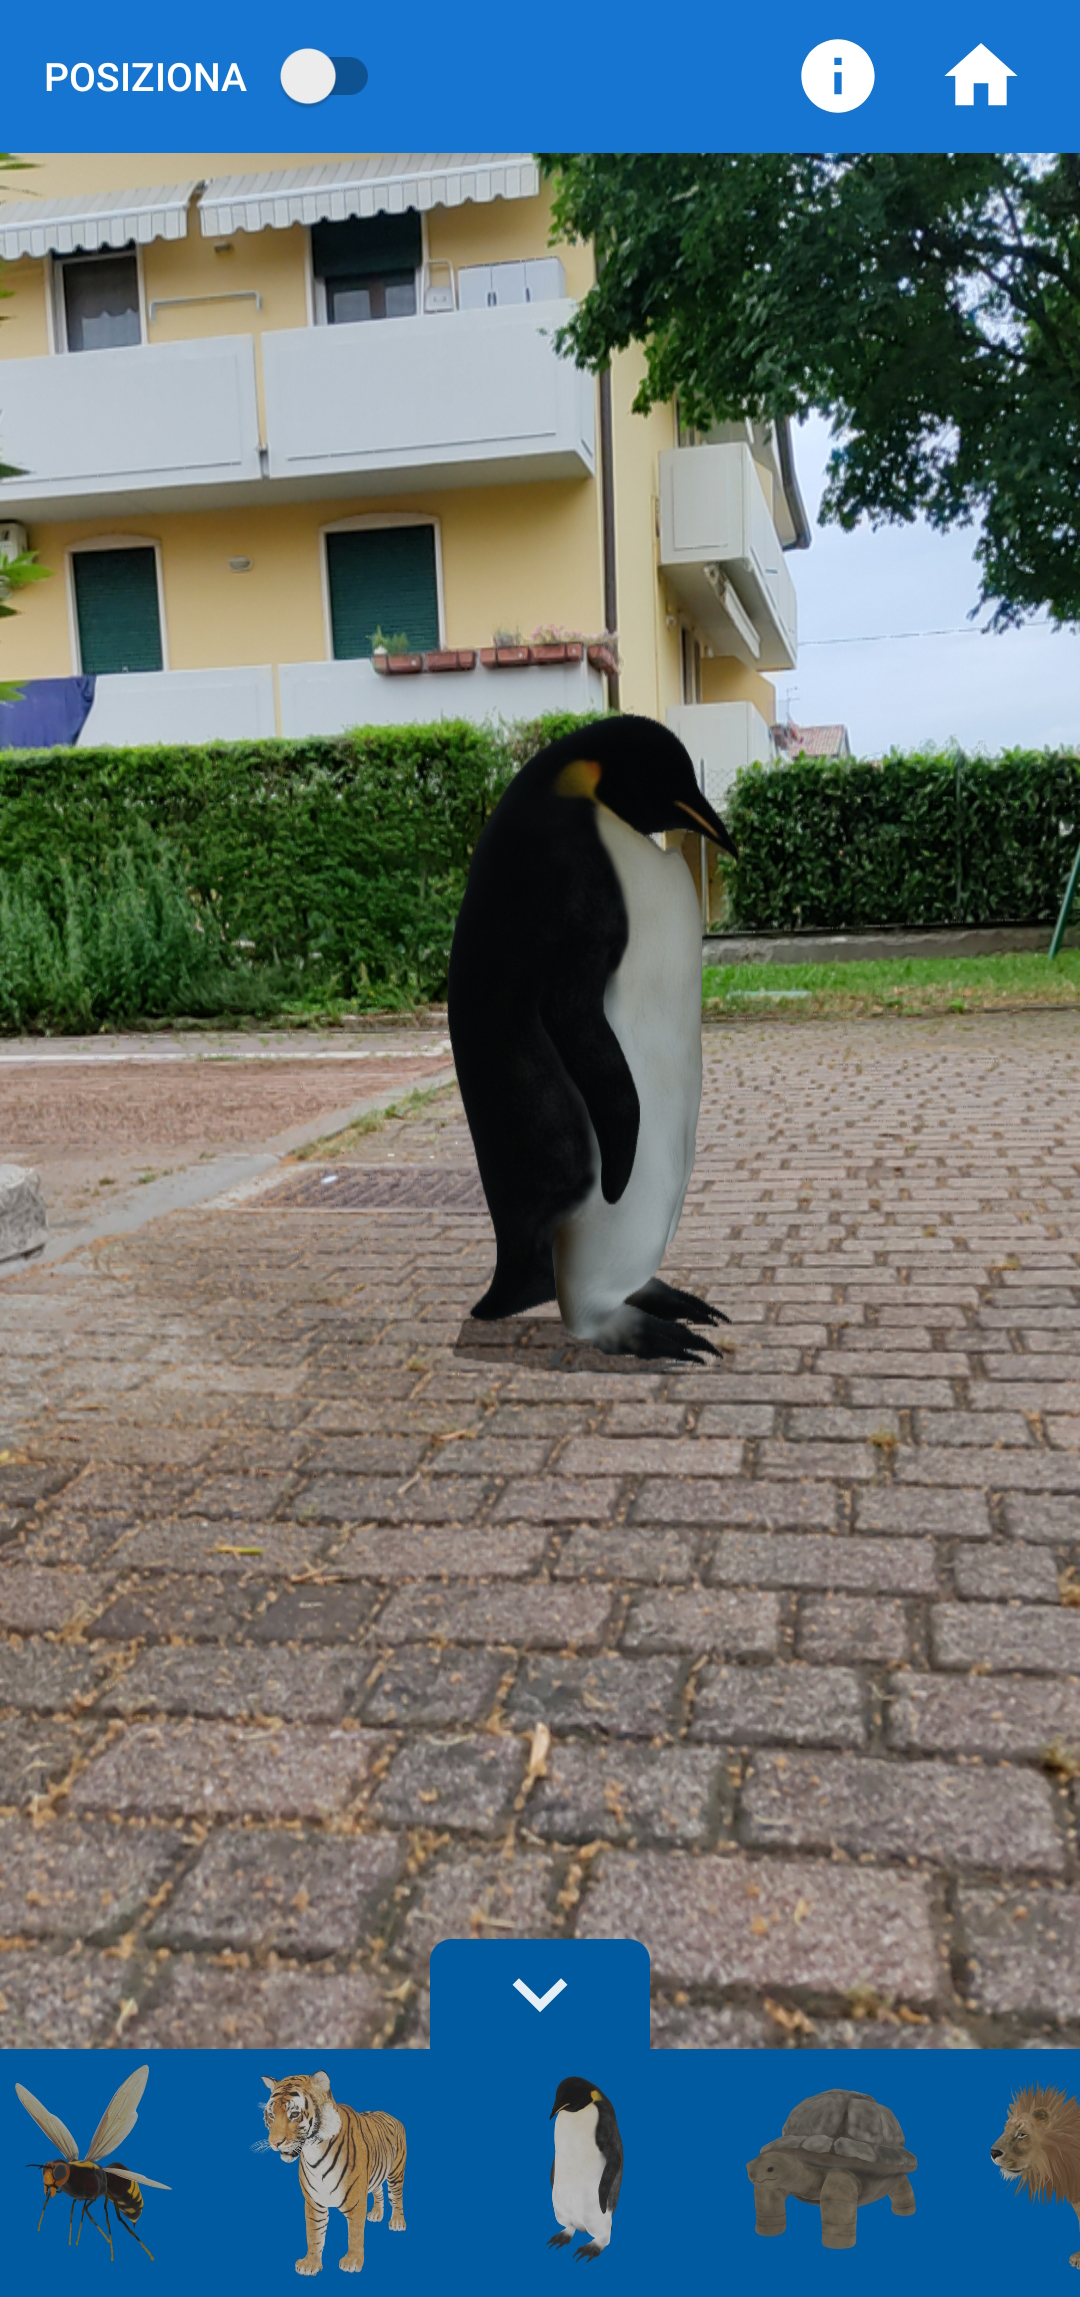
\includegraphics[width=0.3\textwidth]{../../resources/images/AnchorTrackable/pingangolo1.jpg}}%
			{Fonte: \url{nostra applicazione}}
			\caption{Pinguino da una prima inquadratura laterale}
			\label{fig: pinguino angolo1}
	\end{figure}
	
	\begin{figure}
			\centering
			\copyrightbox[0.5]{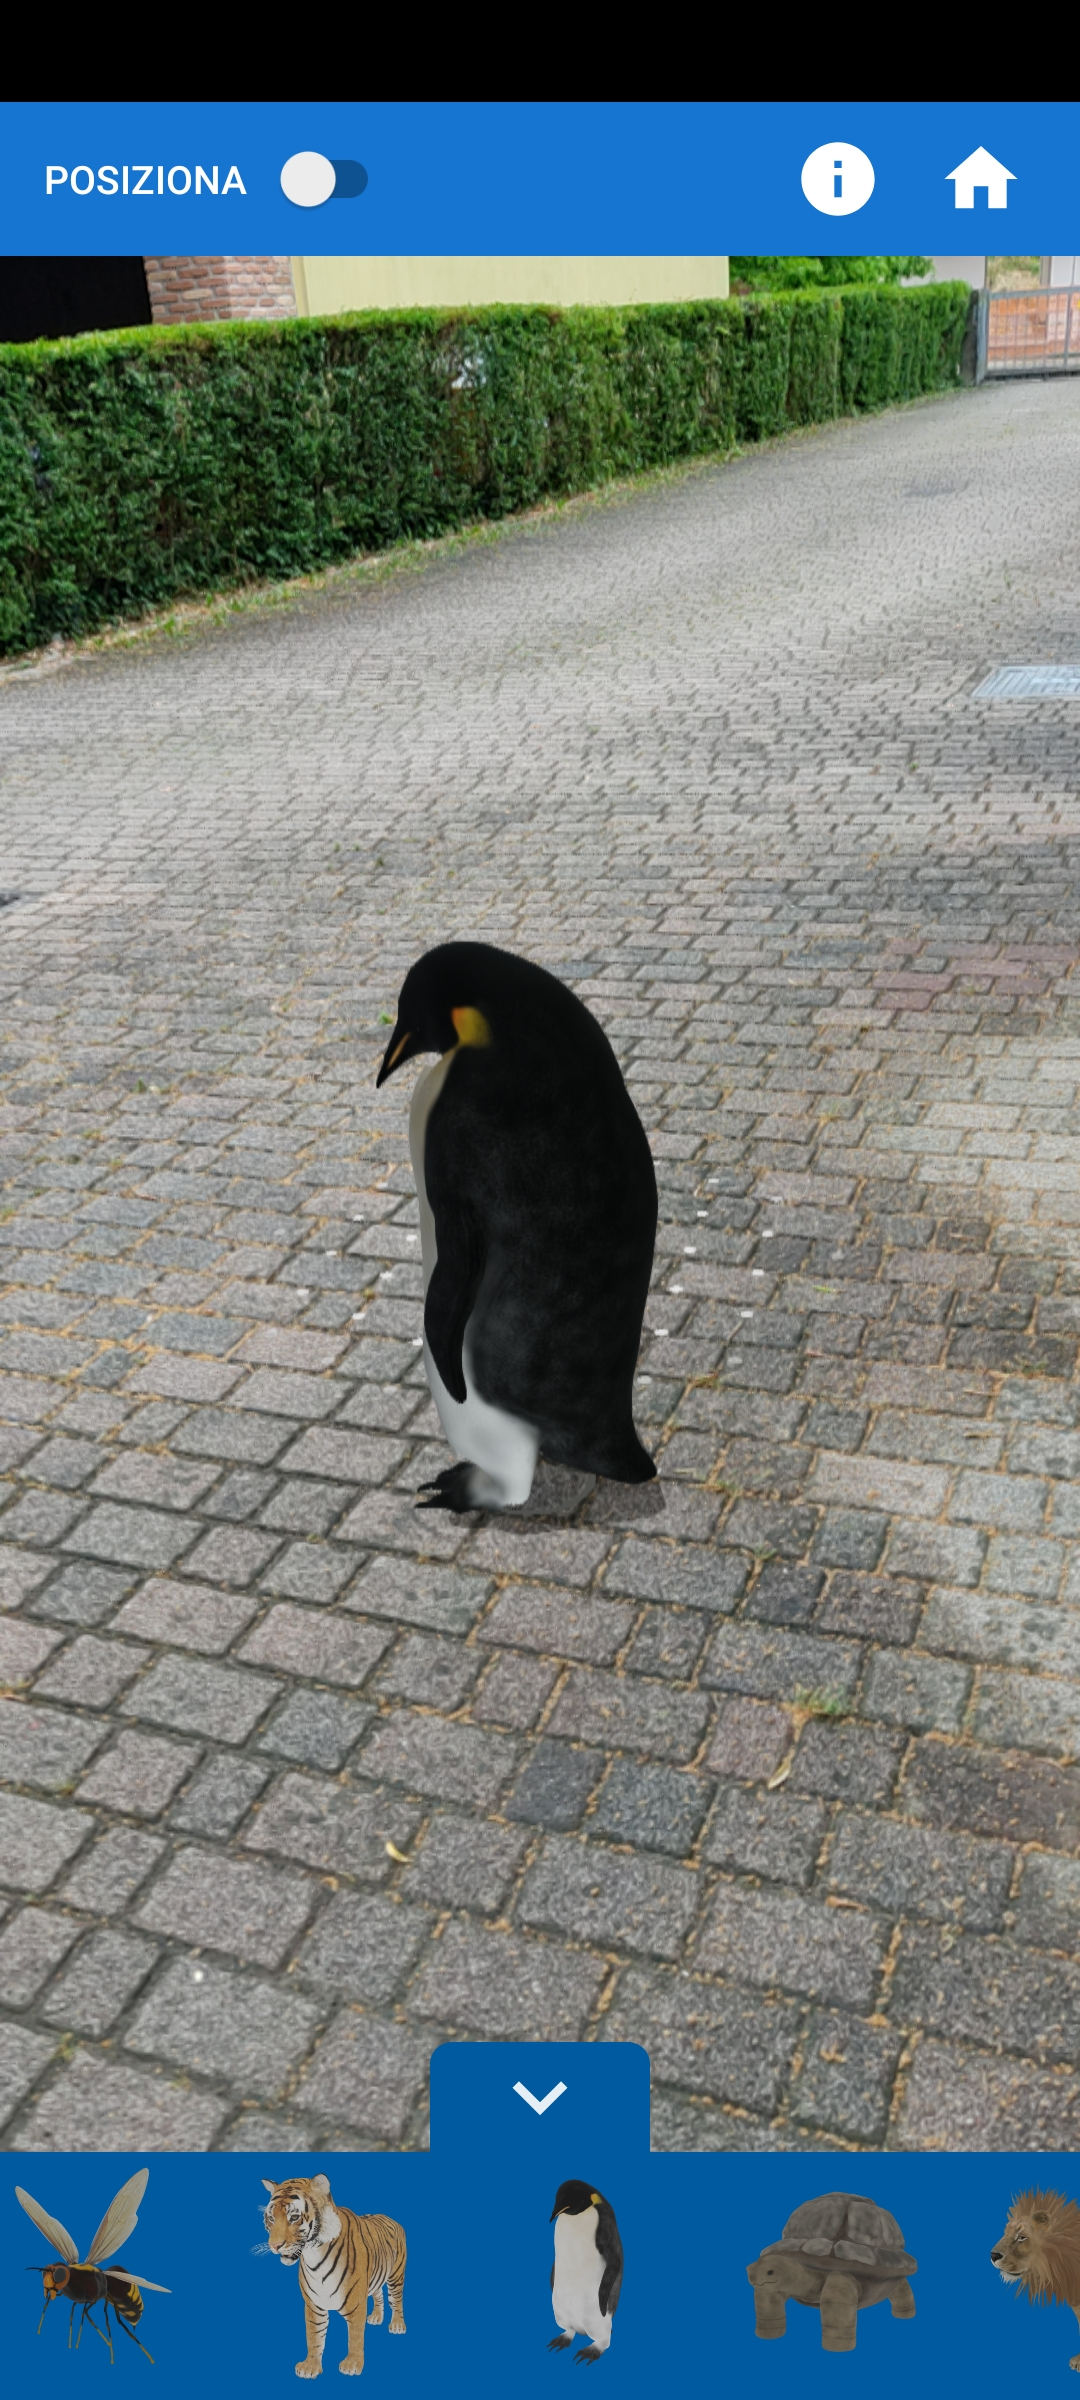
\includegraphics[width=0.3\textwidth]{../../resources/images/AnchorTrackable/pingangolo2.jpg}}%
			{Fonte: \url{nostra applicazione}}
			\caption{Pinguino da una seconda inquadratura laterale}
			\label{fig: pinguino angolo1}
	\end{figure}
		

\end{document}